\chapter{Trạng thái, phép đo và không gian vectơ phức}

\lectureoverview{Cơ học lượng tử khởi đầu bằng việc thay đổi điều ta hiểu là một trạng thái. Trước hết ta tách ra khuôn mẫu cổ điển của các trạng thái và sự cập nhật tất định, rồi dùng một thí nghiệm spin hai kết cục để phơi bày sự thất bại của nó. Câu trả lời toán học là một không gian vectơ phức được trang bị các vectơ đối ngẫu, tích trong, chuẩn và tính trực giao.}

\section{Khuôn mẫu cổ điển: trạng thái và cập nhật}

Bắt đầu với một hệ kín, ít nhất là tạm thời được cô lập khỏi mọi thứ khác. Ở đây, từ \emph{hệ} là một khái niệm nguyên thủy: nó có nghĩa là đối tượng mà ta muốn dự đoán lịch sử của nó. Một \emph{trạng thái} là mọi điều phải biết tại một thời điểm để có thể đưa ra dự đoán đó. Cơ học cổ điển cung cấp một quy luật cập nhật một trạng thái thành trạng thái kế tiếp.

Đối với đồng xu trừu tượng đơn giản nhất,
\begin{equation}
  \mathcal S_{\mathrm{coin}}=\{H,T\}.
\end{equation}
Một quy luật khả dĩ nói rằng không có gì xảy ra:
\begin{equation}
  H\longmapsto H,
  \qquad
  T\longmapsto T.
\end{equation}
Một quy luật khác luân phiên hai trạng thái:
\begin{equation}
  H\longmapsto T,
  \qquad
  T\longmapsto H.
\end{equation}
Các ví dụ này là sơ đẳng, nhưng chúng bộc lộ kiến trúc của một lý thuyết cổ điển:
\begin{equation}
  s(t)\longmapsto s(t+\Delta t).
\end{equation}
Một khi \(s(t)\) đã biết, sự cập nhật là tất định.

Mẫu hình ấy vẫn còn nguyên khi không gian trạng thái là liên tục. Một hạt chuyển động trên một đường thẳng cần cả vị trí lẫn động lượng của nó,
\begin{equation}
  s=(q,p),
\end{equation}
nên không gian trạng thái của nó là mặt phẳng pha. Số trạng thái khả dĩ nay đã trở thành vô hạn, và các phương trình có thể được viết bằng ngôn ngữ tao nhã của các Lagrangian, Hamiltonian và ngoặc Poisson, nhưng ý tưởng nền tảng vẫn không thay đổi. Trạng thái tại một thời điểm chứa điều cần thiết để dự đoán trạng thái tại một thời điểm khác.

\section{Trừu tượng trước trực quan hóa}

Chuyển động cổ điển tương đối dễ hình dung vì các khái niệm của nó được rút ra từ kinh nghiệm thông thường. Lợi thế ấy biến mất khi các đối tượng liên quan quá nhỏ, vận tốc quá lớn, hoặc số chiều của không gian trạng thái quá cao. Không ai thực sự trực quan hóa chuyển động của một electron, không-thời gian bốn chiều hay một không gian mười chiều. Đây không phải là một thiếu sót riêng của người mới học. Trực giác thị giác của con người được hình thành cho thế giới ba chiều hằng ngày.

Ngay cả những trường hợp có vẻ đơn giản hơn cũng cho thấy giới hạn ấy. Điều ta gọi là hình vẽ của một không gian cong hai chiều thường là một mặt được nhúng trong ba chiều. Một đường một chiều được vẽ như một nét trong một mặt phẳng. Hình ảnh ấy âm thầm đưa vào không gian bao quanh mà hệ thị giác của ta biết cách vận hành.

Cách khắc phục không phải là áp đặt một hình dung cổ điển lên thứ vật lý còn xa lạ. Đó là học cấu trúc trừu tượng và để một trực giác mới lớn lên từ những thao tác đúng. Tọa độ ba chiều \((x,y,z)\) trở thành tọa độ bốn chiều \((x,y,z,w)\) bằng cách thêm một ký hiệu và mở rộng các quy tắc, chứ không phải bằng cách có thêm một cơ quan thị giác mới. Cơ học lượng tử đòi hỏi cùng một tính kỷ luật như vậy. Coi nó như một mô hình cơ học kỳ lạ của những vật cổ điển bé nhỏ sẽ lặp đi lặp lại cho ra đáp án sai.

\begin{remark}Trực giác toán học vẫn phát triển. Chỉ là nó không giống với việc nhìn thấy một con sóng trên đại dương hay một mũi tên trong không gian thông thường. Đại số trở nên quen thuộc vì các quan hệ của nó được dùng một cách nhất quán.
\end{remark}

\section{Không gian trạng thái cổ điển và logic cổ điển}

Đối với một hệ cổ điển, không gian trạng thái là một tập hợp. Một con súc sắc trừu tượng có
\begin{equation}
  \mathcal S_{\mathrm{die}}=\{1,2,3,4,5,6\}.
\end{equation}
Một con súc sắc thật có liên tục nhiều tư thế định hướng, nhưng con súc sắc lý tưởng hóa được dùng ở đây chỉ có sáu nhãn này. Một hạt trên một đường thẳng có tập vô hạn liên tục
\begin{equation}
  \mathcal S_{\mathrm{particle}}
  =
  \{(q,p)\mid q,p\in\mathbb R\}.
\end{equation}
Hữu hạn hay vô hạn, mỗi không gian trạng thái cổ điển đều là một tập hợp các khả năng phân biệt lẫn nhau.

Một mệnh đề về hệ chọn ra một tập con của những khả năng đó. Đối với con súc sắc, đặt
\begin{align}
  P_{\mathrm{odd}}&=\{1,3,5\},\\
  P_{\leq 3}&=\{1,2,3\}.
\end{align}
Mệnh đề \emph{lẻ và không lớn hơn ba} tương ứng với giao của chúng:
\begin{equation}
  P_{\mathrm{odd}}\cap P_{\leq 3}=\{1,3\}.
\end{equation}
Mệnh đề tuyển theo nghĩa bao hàm \emph{lẻ hoặc không lớn hơn ba} tương ứng với hợp của chúng:
\begin{equation}
  P_{\mathrm{odd}}\cup P_{\leq 3}
  =
  \{1,2,3,5\}.
\end{equation}
Vì vậy, phép hội và phép tuyển trong logic cổ điển có dạng lý thuyết tập hợp
\begin{equation}
  P\wedge Q\longleftrightarrow P\cap Q,
  \qquad
  P\vee Q\longleftrightarrow P\cup Q.
\end{equation}
Nếu các tập con không giao nhau thì không có trạng thái nào làm cho cả hai mệnh đề cùng đúng.

Logic này gắn với quan niệm cổ điển về trạng thái. Cơ học lượng tử thay thế tập các lựa chọn cổ điển bằng một đối tượng toán học khác: một không gian vectơ. Chỉ trong một giới hạn cổ điển thích hợp thì mô tả bằng không gian vectơ mới xử sự gần đúng như một tập các cấu hình loại trừ lẫn nhau. Trước khi xây dựng không gian ấy, ta cần một thí nghiệm khiến sự thay thế đó trở nên không thể tránh khỏi.

\section{Hệ lượng tử đơn giản nhất}

Đối tượng tương tự lượng tử của đồng xu trừu tượng là một hệ hai kết cục gọi là \emph{qubit}. Các khả năng được đo của nó lúc đầu có thể gắn nhãn là ngửa và sấp, nhưng một nhãn số thì hữu ích hơn:
\begin{equation}
  \sigma\in\{+1,-1\}.
\end{equation}
Ba ký hiệu sẽ được dùng song song:
\begin{equation}
  H\longleftrightarrow \sigma=+1\longleftrightarrow\uparrow,
  \qquad
  T\longleftrightarrow \sigma=-1\longleftrightarrow\downarrow.
\end{equation}
Lúc đầu các mũi tên chỉ là tên gọi. Chưa hề giả định bất kỳ vectơ hình học thông thường nào.

\begin{figure}[htbp]
  \centering
  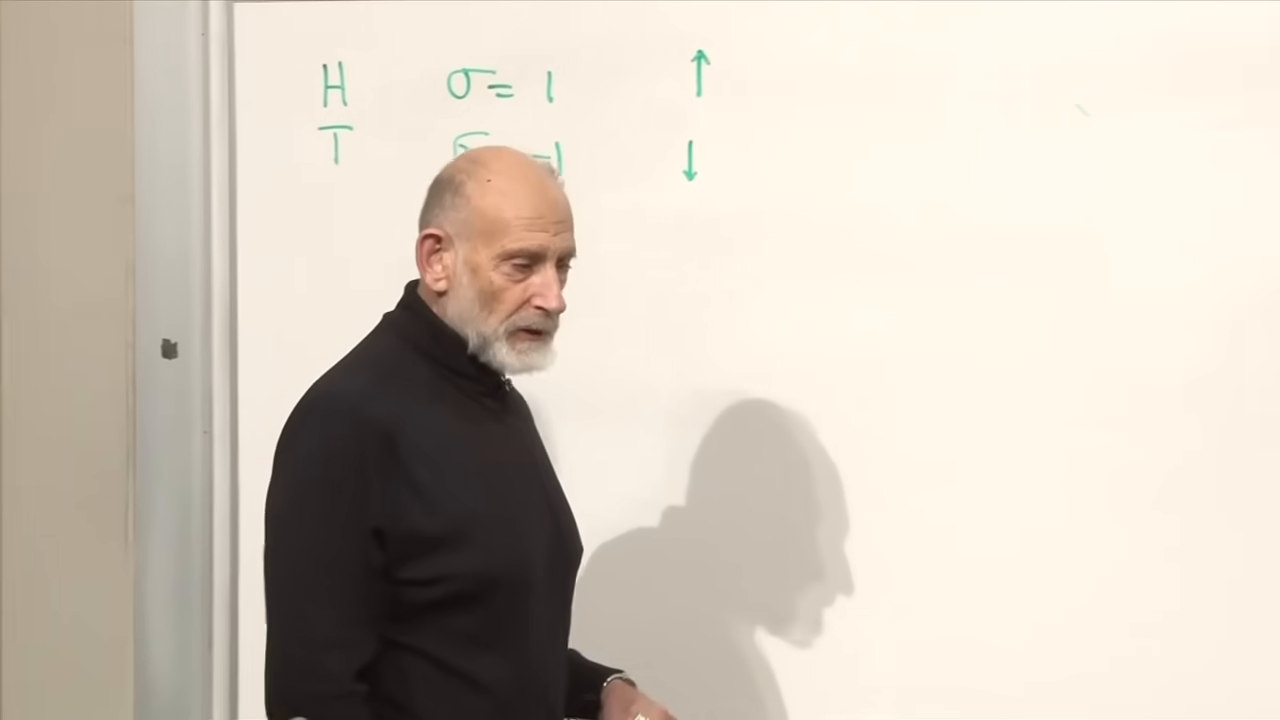
\includegraphics[width=0.78\textwidth]{lecture_01_figure_02.png}
  \caption{Trên bảng, giảng viên đưa vào các nhãn tương đương \(H/T\), \(\sigma=\pm1\) và các mũi tên lên/xuống. Ban đầu các mũi tên là ký hiệu, không phải là một mô hình cổ điển.}
  \lectureframe{00:22:44}
\end{figure}

\begin{classroomqa}
\audiencequestion{Ngửa và sấp có liên quan gì đến hệ vật lý?}
\lecturerresponse{Không gì ngoài việc cung cấp hai tên gọi quen thuộc. Qubit có hai kết cục khả dĩ cho phép đo này; ngửa và sấp chỉ là các nhãn giữ chỗ. Các nhãn \(\pm1\) được chọn vì chúng có thể đi vào các phương trình.}
\end{classroomqa}

\subsection{Thiết bị như một hộp đen}

Một thí nghiệm đòi hỏi một hệ thứ hai, là thiết bị \(A\). Tạm thời, nó là một hộp đen trừu tượng có ba đặc điểm:
\begin{enumerate}
  \item nó có một định hướng trong không gian, được đánh dấu bằng \emph{mặt này hướng lên trên};
  \item nó có một cảm biến có thể tương tác với qubit;
  \item nó có một màn hiển thị ban đầu để trống và sau đó hiện \(+1\) hoặc \(-1\).
\end{enumerate}
Chi tiết của bộ dò được cố ý để lại sau. Một bộ dò tốt được xác định theo nghĩa thao tác bởi mối liên hệ đáng tin cậy giữa hệ và bản ghi của nó. Người quan sát không nhất thiết phải nhìn vào lúc tương tác xảy ra; thiết bị có thể ghi lại kết quả và được đọc sau.

Giả sử màn hiển thị báo \(+1\). Đặt lại thiết bị về trạng thái để trống và lặp lại ngay cùng phép đo ấy, trước khi bất kỳ diễn biến độc lập nào kịp tác động. Một bộ dò trung thực sẽ lại báo \(+1\). Nếu kết quả đầu tiên là \(-1\), thì các lần lặp lại tức thời cũng tiếp tục báo \(-1\):
\begin{equation}
\begin{aligned}
  +1&\longrightarrow +1\longrightarrow +1\longrightarrow\cdots,\\
  -1&\longrightarrow -1\longrightarrow -1\longrightarrow\cdots.
\end{aligned}
\end{equation}
Vì vậy, phép đo thứ nhất có thể được xem như một sự \emph{chuẩn bị}. Nó để qubit lại trong một trạng thái mà ở đó việc lặp lại ngay chính phép đo ấy cho một kết quả xác định.

Tính lặp lại này không phải là một lời bình triết học tùy ý. Không có nó thì sẽ không có cách nào theo nghĩa thao tác để xác nhận một phép đo. Một thiết bị bị lỗi có thể không lặp lại được kết quả của nó, nhưng khi đó nó không thực hiện phép đo lý tưởng đang được định nghĩa.

\begin{classroomqa}
\audiencequestion{Đây đã là sự sụp đổ của hàm sóng chưa?}
\lecturerresponse{Có thể đưa cách nói đó vào sau. Ở giai đoạn này, phát biểu theo nghĩa thao tác là đủ: một phép đo tạo ra một kết quả và chuẩn bị một trạng thái mà trong đó cùng phép đo tức thời ấy tái tạo lại kết quả đó. Việc đặt tên cho quá trình này vẫn chưa giải thích nó.}
\end{classroomqa}

\section{Định hướng và sự thất bại của con trỏ cổ điển}

Hãy chuẩn bị qubit sao cho thiết bị ở tư thế thẳng đứng cho kết quả \(+1\). Quay thiết bị đi \(180^\circ\) và lặp lại phép đo. Kết quả bây giờ là \(-1\). Các phép đo lặp lại với thiết bị đảo ngược xác nhận \(-1\), còn khi dựng thiết bị thẳng đứng trở lại thì \(+1\) được khôi phục.

Kết quả ấy bộc lộ tính định hướng thật sự. Ký hiệu lên/xuống không hoàn toàn tùy ý: đảo ngược bộ dò thì dấu cũng đảo. Người ta dễ bị cám dỗ kết luận rằng qubit đơn giản chỉ là một vectơ nhỏ và bộ dò đo thành phần của vectơ đó dọc theo trục riêng của nó. Sự cám dỗ ấy phải được kiểm tra chứ không được tin ngay.

\begin{figure}[htbp]
  \centering
  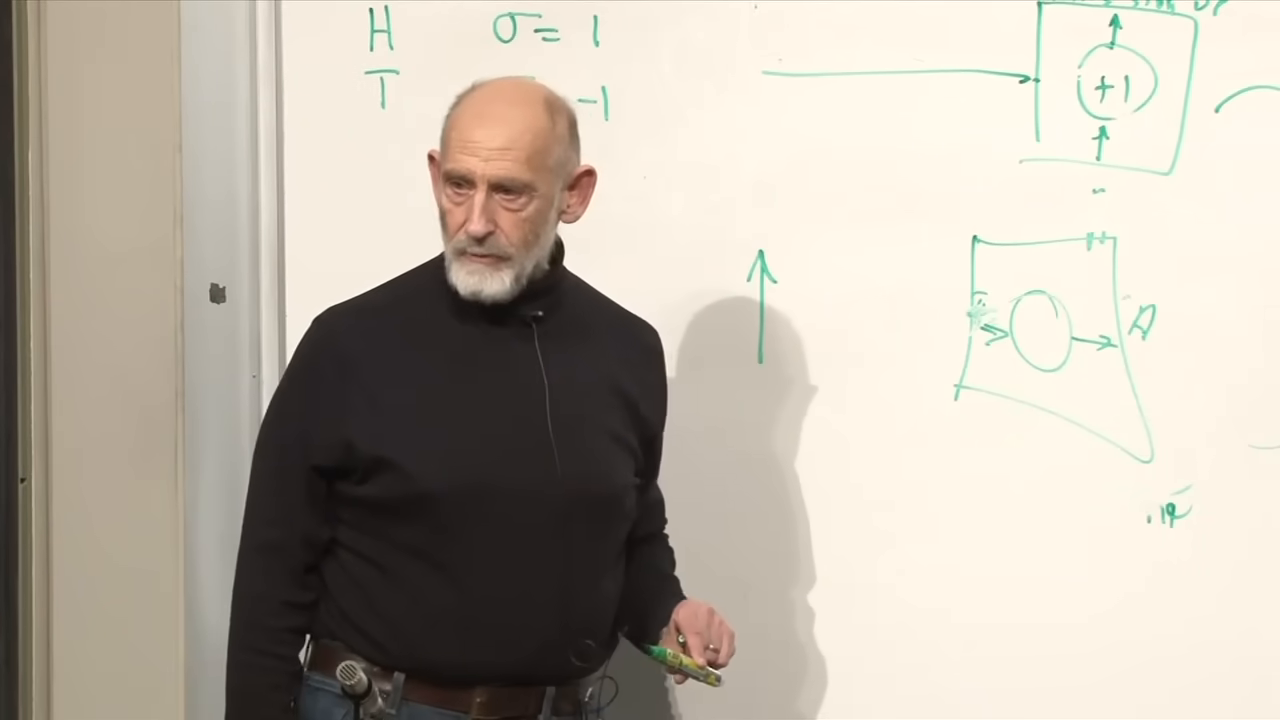
\includegraphics[width=0.82\textwidth]{lecture_01_figure_03.png}
  \caption{Một phép chuẩn bị hướng lên và các bộ phân tích có định hướng khác nhau trên bảng. Về sau trong lớp đã sửa hướng của một mũi tên phấn; trong lập luận chỉ trục của bộ phân tích mới quan trọng.}
  \lectureframe{00:36:21}
\end{figure}

\subsection{Một phép đo theo phương ngang}

Quay bộ dò đi \(90^\circ\). Nếu qubit đã chuẩn bị là một con trỏ hướng lên thông thường, thì thành phần của nó dọc theo trục ngang của bộ dò sẽ bằng không:
\begin{equation}
  \hat{\mathbf x}\cdot\hat{\mathbf z}=0.
\end{equation}
Thiết bị lượng tử không bao giờ báo bằng không. Mỗi phép thử riêng lẻ đều cho \(+1\) hoặc \(-1\).

\begin{figure}[htbp]
  \centering
  \resizebox{\linewidth}{!}{%
  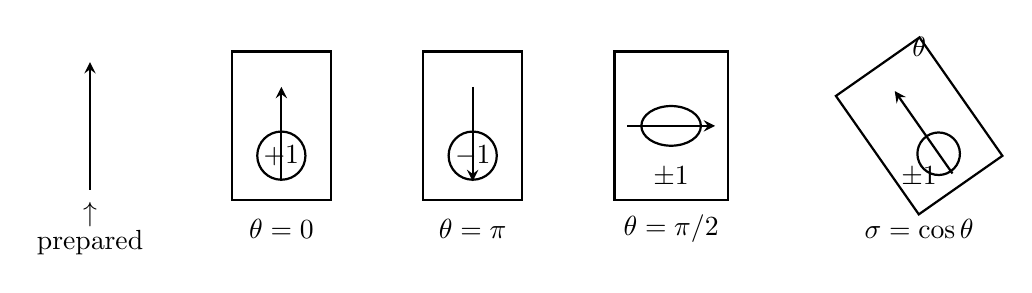
\begin{tikzpicture}[>=stealth,thick,scale=0.90]
    \draw[->] (0,0)--(0,1.8);
    \node at (0,-0.35) {\(\uparrow\)};
    \node at (0,-0.75) {prepared};

    \draw (2.0,-0.15) rectangle (3.4,1.95);
    \draw (2.7,0.48) circle (0.34);
    \draw[->] (2.7,0.12)--(2.7,1.45);
    \node at (2.7,0.48) {\(+1\)};
    \node at (2.7,-0.55) {\(\theta=0\)};

    \draw (4.7,-0.15) rectangle (6.1,1.95);
    \draw (5.4,0.48) circle (0.34);
    \draw[->] (5.4,1.45)--(5.4,0.12);
    \node at (5.4,0.48) {\(-1\)};
    \node at (5.4,-0.55) {\(\theta=\pi\)};

    \draw (7.4,-0.15) rectangle (9.0,1.95);
    \draw (8.2,0.90) ellipse (0.42 and 0.28);
    \draw[->] (7.58,0.90)--(8.82,0.90);
    \node at (8.2,0.18) {\(\pm1\)};
    \node at (8.2,-0.55) {\(\theta=\pi/2\)};

    \begin{scope}[shift={(11.7,0.90)},rotate=35]
      \draw (-0.72,-1.02) rectangle (0.72,1.02);
      \draw (0,-0.48) circle (0.30);
      \draw[->] (0,-0.82)--(0,0.60);
    \end{scope}
    \node at (11.7,0.18) {\(\pm1\)};
    \node at (11.7,-0.55) {\(\expect{\sigma}=\cos\theta\)};
    \node at (11.7,2.02) {\(\theta\)};
  \end{tikzpicture}
  }%
  \caption{Phục dựng chuỗi bộ phân tích. Một phép quay làm thay đổi thống kê, chứ không bao giờ làm thay đổi tập các kết cục riêng lẻ.}
\end{figure}

Chuẩn bị một tập lớn qubit bằng thiết bị thẳng đứng, và giữ lại những qubit cho kết quả \(+1\). Đo mỗi qubit được giữ lại đúng một lần bằng thiết bị theo phương ngang. Một nửa số phép thử cho \(+1\), một nửa cho \(-1\), và giá trị trung bình của cả tập hợp bằng không:
\begin{equation}
  \expect{\sigma}_{\pi/2}=0.
\end{equation}
Giá trị trung bình ấy giống với thành phần ngang bằng không của một con trỏ cổ điển, nhưng các bản ghi riêng lẻ thì không. Giá trị cổ điển \(0\) đã được thay thế bằng một sự cân bằng thống kê giữa hai kết cục rời rạc.

\begin{classroomqa}
\audiencequestion{Điều gì xảy ra nếu giữ lại chính qubit đó thay vì loại bỏ nó sau phép đo theo phương ngang?}
\lecturerresponse{Giả sử kết quả ngang đầu tiên của nó là \(+1\). Lặp lại phép đo theo phương ngang trên chính qubit ấy sẽ lại cho \(+1\) hết lần này đến lần khác. Phép đo ngang thứ nhất đã chuẩn bị nó theo trục ngang. Muốn thu được thống kê chia đều, ta phải lặp lại toàn bộ thí nghiệm chuẩn bị-và-đo trên nhiều qubit, chứ không phải liên tục xác nhận một kết quả.}
\end{classroomqa}

\subsection{Các phép chuẩn bị không tương thích}

Thứ tự các trục là quan trọng. Hãy chuẩn bị \(+1\) theo phương thẳng đứng, rồi đo theo phương ngang. Kết quả ngang đầu tiên là ngẫu nhiên. Một khi đã thu được một kết quả ngang, thì các lần lặp lại ngang ngay sau đó là xác định. Bây giờ quay bộ dò trở lại trục thẳng đứng. Kết quả theo phương thẳng đứng lại ngẫu nhiên.

Theo ký hiệu, trong đó \(M_z\) và \(M_x\) ký hiệu các phép đo dọc theo hai trục,
\begin{equation}
\begin{aligned}
  M_z&:+1,\\
  M_x&:\pm1,\\
  M_x&:\text{same result},\\
  M_z&:\pm1.
\end{aligned}
\end{equation}
Phép đo \(x\) ở giữa không chỉ đơn thuần bộc lộ một thành phần ngang mà vẫn bảo toàn trạng thái thẳng đứng ban đầu. Nó đã chuẩn bị một trạng thái mới, và tính xác định thẳng đứng ban đầu đã mất.

\begin{classroomqa}
\audiencequestion{Bộ dò có nhớ câu trả lời đầu tiên không? Làm sao nó biết qubit được đưa vào là cùng qubit ấy hay là một qubit mới?}
\lecturerresponse{Tính lặp lại là một tính chất của qubit được đo, không phải là một phép so sánh ký ức ẩn do bộ dò thực hiện. Sau một phép đo, qubit ở trong một trạng thái cho cùng câu trả lời đối với cùng phép đo tức thời ấy. Nếu đưa vào một qubit được chuẩn bị khác đi, kết quả sẽ phụ thuộc vào sự chuẩn bị đó. Việc theo dõi xem hệ vật lý nào đang được đo là công việc ghi chép phòng thí nghiệm thông thường.}
\end{classroomqa}

\begin{classroomqa}
\audiencequestion{Vậy chính việc quan sát chuẩn bị qubit cụ thể đó?}
\lecturerresponse{Đúng. Một khi phép đo ấy đã chuẩn bị qubit, thì chính phép đo đó sẽ cho cùng câu trả lời cho đến khi có một diễn biến khác hoặc một phép đo không tương thích xen vào.}
\end{classroomqa}

\section{Một bộ phân tích quay một góc tùy ý}

Hãy để trục bộ dò hợp một góc \(\theta\) với trục mà theo đó tập hợp đã được chuẩn bị. Mỗi phép thử vẫn cho
\begin{equation}
  \sigma=\pm1.
\end{equation}
Các tần suất tương đối biến thiên theo góc sao cho giá trị trung bình là
\begin{equation}
  \expect{\sigma}_{\theta}=\cos\theta.
  \label{eq:qml1-cosine-mean}
\end{equation}
Các trường hợp giới hạn là
\begin{align}
  \expect{\sigma}_{0}&=+1,\\
  \expect{\sigma}_{\pi/2}&=0,\\
  \expect{\sigma}_{\pi}&=-1.
\end{align}
Gần \(\theta=0\), phần lớn các kết cục là \(+1\), chỉ thỉnh thoảng mới có \(-1\). Gần \(\theta=\pi\), phần lớn là \(-1\), chỉ thỉnh thoảng mới có \(+1\).

\begin{figure}[htbp]
  \centering
  \includegraphics[width=0.82\textwidth]{lecture_01_figure_04.png}
  \caption{Bảng viết thực tế cho thí nghiệm góc tùy ý: một tập hợp được chuẩn bị theo phương thẳng đứng đi vào một bộ phân tích nghiêng một góc \(\theta\).}
  \lectureframe{00:48:55}
\end{figure}

Đại lượng biến thiên trơn mang tính vectơ là giá trị trung bình của tập hợp, không phải kết quả đơn lẻ. Nếu \(p_+(\theta)\) và \(p_-(\theta)\) là hai xác suất, thì
\begin{equation}
  p_+ + p_-=1,
  \qquad
  p_+-p_-=\cos\theta.
\end{equation}
Do đó,
\begin{equation}
\begin{aligned}
  p_+(\theta)&=\frac{1+\cos\theta}{2}
  =\cos^2\frac{\theta}{2},\\
  p_-(\theta)&=\frac{1-\cos\theta}{2}
  =\sin^2\frac{\theta}{2}.
\end{aligned}
  \label{eq:qml1-half-angle-probabilities}
\end{equation}
\editorialnote{Bài giảng nêu hai kết quả và giá trị trung bình của chúng là \(\cos\theta\). Phương trình~\eqref{eq:qml1-half-angle-probabilities} là hệ quả đại số trực tiếp của những phát biểu ấy và làm hiển lộ tường minh quy luật tần suất được ngụ ý.}

\begin{classroomqa}
\audiencequestion{Một tập hợp các qubit chưa được chuẩn bị có cũng sẽ cho giá trị trung bình \(\cos\theta\) không?}
\lecturerresponse{Không có phương nào cụ thể được chọn ra trong một tập hợp không phân cực, nên giá trị trung bình của nó bằng không. Sự phụ thuộc vào \(\theta\) nói tới một tập hợp trước hết được chuẩn bị dọc theo một trục xác định.}
\end{classroomqa}

\begin{classroomqa}
\audiencequestion{Vì sao cần cả một tập hợp nếu qubit không có động lực học xen giữa?}
\lecturerresponse{Phép đo nghiêng đầu tiên trên một qubit cho một mẫu duy nhất. Mọi lần lặp lại ngay sau đó trên chính qubit ấy chỉ xác nhận mẫu đó. Các phép thử độc lập đòi hỏi những qubit được chuẩn bị giống hệt nhau, mỗi qubit được đo một lần bằng bộ phân tích nghiêng.}
\end{classroomqa}

\begin{classroomqa}
\audiencequestion{Có những mẫu hình hay tương quan bậc cao nào trong chuỗi các dấu cộng và dấu trừ không?}
\lecturerresponse{Đối với thí nghiệm này, các phép thử riêng rẽ được giả định là độc lập và không tương quan. Xác suất của từng phép thử phụ thuộc vào \(\theta\), nhưng không có thêm mẫu hình sắp xếp nào được khẳng định ở đây.}
\end{classroomqa}

\subsection{Những gì đã được lý tưởng hóa}

Hiện thời, thiết bị được xem như một đối tượng cổ điển có định hướng điều chỉnh liên tục và đầu ra rời rạc. Sự phân chia giữa \emph{hệ} và \emph{bộ dò} này chỉ là tạm thời. Bản thân bộ dò cũng là một hệ vật lý và rốt cuộc cũng phải tuân theo cơ học lượng tử. Một mô tả đầy đủ sẽ xét hệ và thiết bị cùng nhau, nhưng điều đó đòi hỏi những công cụ hiện chưa có sẵn.

\begin{classroomqa}
\audiencequestion{Bản thân bộ dò có chỉ là một hệ hai trạng thái khác không?}
\lecturerresponse{Nó có các trạng thái vật lý và rốt cuộc phải được đưa vào mô tả lượng tử. Hiện giờ ta giữ một sự tách biệt mang tính thao tác: qubit là đối tượng được mô tả bằng cơ học lượng tử, còn bộ dò có định hướng cung cấp một bản ghi cổ điển ổn định. Về sau, hệ ghép phải được phân tích như các hệ lượng tử tương tác.}
\end{classroomqa}

\begin{classroomqa}
\audiencequestion{Việc thay đổi trục mà quanh đó bộ dò được quay có đưa vào nhiều cấu trúc hơn chỉ một góc duy nhất được minh họa ở đây không?}
\lecturerresponse{Có, câu chuyện đầy đủ trong ba chiều phong phú hơn. Phép quay trong một mặt phẳng là lát cắt đơn giản nhất của nó và phù hợp với cách xử lý đầy đủ hơn sẽ đến sau.}
\end{classroomqa}

\begin{classroomqa}
\audiencequestion{Bộ dò có thể trả về một giá trị liên tục giữa \(-1\) và \(+1\) không?}
\lecturerresponse{Định hướng của nó biến thiên liên tục, nhưng mỗi số đọc qubit lý tưởng riêng lẻ vẫn là \(+1\) hoặc \(-1\). Tính liên tục xuất hiện ở các xác suất và giá trị trung bình khi định hướng thay đổi, chứ không ở từng kết quả riêng lẻ.}
\end{classroomqa}

\section{Mũi tên chỉ và vectơ trừu tượng}

Các dữ kiện thực nghiệm giờ tạm thời được tách khỏi phần toán học. Một mũi tên thông thường trong không gian vật lý sẽ được gọi là một \emph{mũi tên chỉ}. Một vectơ toán học là khái niệm tổng quát hơn: nó là một phần tử của một không gian vectơ và không nhất thiết chỉ theo bất kỳ hướng nào trong không gian thông thường.

\begin{definition}
Một không gian vectơ phức \(V\) là một tập hợp các vectơ mà trên đó phép cộng vectơ và phép nhân với vô hướng phức được xác định và thỏa mãn các quy tắc tuyến tính thông thường. Cụ thể, với \(u,v,w\in V\) và \(a,b\in\mathbb C\),
\begin{align}
  u+v&=v+u,\\
  (u+v)+w&=u+(v+w),\\
  a(u+v)&=au+av,\\
  (a+b)u&=au+bu,\\
  (ab)u&=a(bu),\\
  1u&=u.
\end{align}
Có một vectơ không \(0\) và một phần tử đối cộng \(-u\) cho mọi \(u\).
\end{definition}

Thảo luận trên lớp ban đầu chỉ nhấn mạnh các phép toán và tính đóng:
\begin{equation}
\begin{aligned}
  u,v\in V&\Longrightarrow u+v\in V,\\
  a\in\mathbb C,\ u\in V&\Longrightarrow au\in V.
\end{aligned}
\end{equation}
Vectơ không và tính giao hoán sau đó mới được bổ sung để trả lời các câu hỏi. Những tiên đề quen thuộc còn lại chỉ phát biểu tường minh điều vốn đã được dùng khi mô hình vectơ cột cụ thể được đưa vào.

Các số thực tạo thành một không gian vectơ một chiều trên \(\mathbb R\). Các số phức tạo thành một không gian vectơ một chiều trên \(\mathbb C\), và một không gian vectơ hai chiều trên \(\mathbb R\). Các hàm nhận giá trị phức \(\psi(x)\) cũng tạo thành một không gian vectơ phức vì
\begin{equation}
  (\psi+\phi)(x)=\psi(x)+\phi(x),
  \qquad
  (z\psi)(x)=z\psi(x).
\end{equation}
Ví dụ về không gian hàm này sau sẽ trở thành trung tâm, nhưng trước hết các cột hữu hạn làm cho cấu trúc dễ thấy hơn.

\begin{classroomqa}
\audiencequestion{Sự khác nhau giữa một vectơ và một không gian vectơ là gì?}
\lecturerresponse{Vectơ là một phần tử. Không gian vectơ là tập hợp gồm tất cả các phần tử như thế cùng với các quy tắc để cộng chúng và nhân chúng với các vô hướng, cũng như một con số là một đối tượng còn hệ thống số là một tập hợp đi kèm các phép toán.}
\end{classroomqa}

\section{Các cột phức hai thành phần}

Viết một vectơ trừu tượng trong ký hiệu Dirac dưới dạng \(\ket{\alpha}\). Một biểu diễn cụ thể là
\begin{equation}
  \ket{\alpha}
  \longleftrightarrow
  \begin{pmatrix}
    \alpha_1\\
    \alpha_2
  \end{pmatrix},
  \qquad
  \alpha_1,\alpha_2\in\mathbb C.
\end{equation}
Nếu
\begin{equation}
  \ket{\beta}
  \longleftrightarrow
  \begin{pmatrix}
    \beta_1\\
    \beta_2
  \end{pmatrix},
\end{equation}
thì phép cộng và phép nhân vô hướng được xác định theo từng thành phần:
\begin{align}
  \ket{\alpha}+\ket{\beta}
  &\longleftrightarrow
  \begin{pmatrix}
    \alpha_1+\beta_1\\
    \alpha_2+\beta_2
  \end{pmatrix},\\
  z\ket{\alpha}
  &\longleftrightarrow
  \begin{pmatrix}
    z\alpha_1\\
    z\alpha_2
  \end{pmatrix},
  \qquad z\in\mathbb C.
\end{align}

\begin{figure}[htbp]
  \centering
  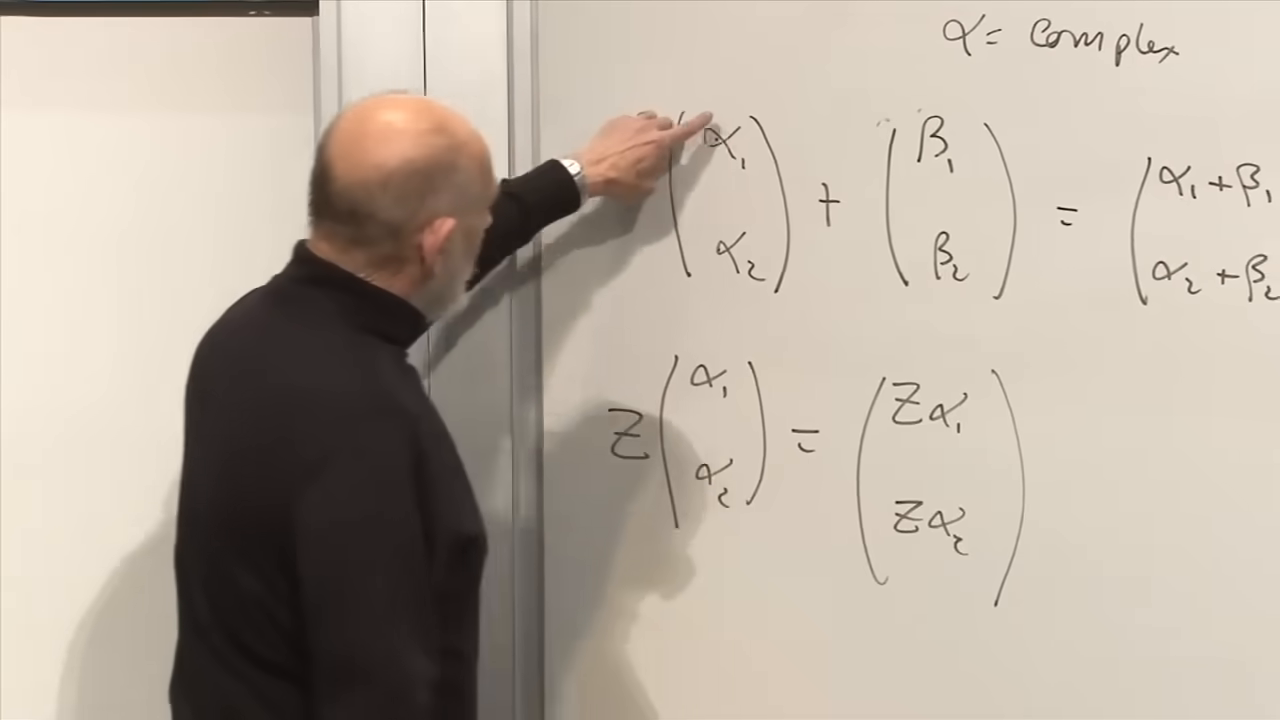
\includegraphics[width=0.88\textwidth]{lecture_01_figure_05.png}
  \caption{Các quy tắc theo từng thành phần để cộng hai cột phức và nhân một cột với một vô hướng phức.}
  \lectureframe{01:14:28}
\end{figure}

Vectơ không là
\begin{equation}
  \ket{0}
  =
  \begin{pmatrix}
    0\\
    0
  \end{pmatrix},
  \qquad
  \ket{\alpha}+\ket{0}=\ket{\alpha}.
\end{equation}
Các cột có ba thành phần tạo thành một không gian vectơ khác, và tương tự như vậy với mọi số thành phần cố định. Một cột hai thành phần không thể cộng với một cột ba thành phần vì hai đối tượng ấy thuộc các không gian khác nhau và không có quy tắc theo từng thành phần nào liên hệ chúng.

\begin{classroomqa}
\audiencequestion{Vectơ cột có phải là một ma trận không?}
\lecturerresponse{Theo thuật ngữ tổng quát, nó là một ma trận có một cột. Trong môn học này, từ \emph{ma trận} thường sẽ có nghĩa là một bảng vuông, còn một bảng một cột sẽ được gọi là một vectơ cột. Sự phân biệt này là về thuật ngữ, không phải bất đồng về đại số.}
\end{classroomqa}

\begin{classroomqa}
\audiencequestion{Thứ tự cộng vectơ có quan trọng không?}
\lecturerresponse{Không. Phép cộng theo từng thành phần thừa hưởng tính giao hoán từ các số phức:
\[
  \ket{\alpha}+\ket{\beta}
  =
  \ket{\beta}+\ket{\alpha}.
\]
Đây là một trong các tiên đề của không gian vectơ.}
\end{classroomqa}

\section{Vectơ đối ngẫu: bra và ket}

Với mỗi ket \(\ket{A}\) có một vectơ tương ứng trong không gian đối ngẫu, viết là \(\bra{A}\). Ánh xạ từ ket sang bra có tính cộng tính nhưng liên hợp các vô hướng phức:
\begin{align}
  \ket{A}+\ket{B}
  &\longleftrightarrow
  \bra{A}+\bra{B},\\
  z\ket{A}
  &\longleftrightarrow
  z^*\bra{A}.
  \label{eq:qml1-antilinear-dual}
\end{align}
Quy tắc thứ hai này là nét phức cốt yếu. Đối ngẫu của một bội vô hướng được nhân với vô hướng liên hợp phức.

\begin{figure}[htbp]
  \centering
  \includegraphics[width=0.86\textwidth]{lecture_01_figure_06.png}
  \caption{Phép tương ứng ket-sang-bra và hai quy tắc của nó: tổng ánh xạ thành tổng, còn phép nhân vô hướng thì bị liên hợp phức.}
  \lectureframe{01:23:15}
\end{figure}

Đối với cách biểu diễn hai thành phần,
\begin{equation}
  \ket{\alpha}
  =
  \begin{pmatrix}
    \alpha_1\\
    \alpha_2
  \end{pmatrix}
  \qquad\Longrightarrow\qquad
  \bra{\alpha}
  =
  \begin{pmatrix}
    \alpha_1^*&\alpha_2^*
  \end{pmatrix}.
  \label{eq:qml1-bra-from-ket}
\end{equation}
Phép liên hợp phức thực hiện sự tương ứng đối ngẫu, và ký hiệu hàng giữ cho hai loại đối tượng phân biệt rõ ràng bằng mắt. Phương trình~\eqref{eq:qml1-bra-from-ket} cũng kiểm chứng trực tiếp Phương trình~\eqref{eq:qml1-antilinear-dual}.

\section{Tích trong}

Cho \(\ket{\alpha}\) và \(\ket{\beta}\), ghép bra ứng với \(\beta\) với ket \(\alpha\):
\begin{equation}
  \braket{\beta}{\alpha}
  =
  \begin{pmatrix}
    \beta_1^*&\beta_2^*
  \end{pmatrix}
  \begin{pmatrix}
    \alpha_1\\
    \alpha_2
  \end{pmatrix}
  =
  \beta_1^*\alpha_1+\beta_2^*\alpha_2.
  \label{eq:qml1-inner-product}
\end{equation}
Từ \emph{bracket} được ghép đúng theo nghĩa đen từ \emph{bra} và \emph{ket}. Đây là phép tương tự phức của tích vô hướng: nhân các thành phần tương ứng rồi cộng lại, với phép liên hợp phức đặt ở phía bra.

\begin{figure}[htbp]
  \centering
  \includegraphics[width=0.88\textwidth]{lecture_01_figure_07.png}
  \caption{Trên bảng, tích trong \(\braket{\beta}{\alpha}\) được tính thành \(\beta_1^*\alpha_1+\beta_2^*\alpha_2\).}
  \lectureframe{01:31:25}
\end{figure}

Hoán đổi hai vectơ cho
\begin{equation}
  \braket{\alpha}{\beta}
  =
  \alpha_1^*\beta_1+\alpha_2^*\beta_2
  =
  \braket{\beta}{\alpha}^{*}.
  \label{eq:qml1-conjugate-symmetry}
\end{equation}
Vì thế, nhìn chung thứ tự là quan trọng, nhưng chỉ thông qua phép liên hợp phức.

\begin{classroomqa}
\audiencequestion{Có thể định nghĩa một tích của các vectơ phức mà không liên hợp một phía không?}
\lecturerresponse{Ta có thể đặt ra một biểu thức song tuyến tính như vậy, nhưng khi đó tích của một vectơ với chính nó không nhất thiết là số thực hay dương. Cấu trúc ấy không phải cấu trúc hữu ích cho cơ học lượng tử. Tích trong có liên hợp, hay Hermite, cho ra chuẩn và cấu trúc xác suất sẽ cần đến.}
\end{classroomqa}

\subsection{Chuẩn và tính dương}

Đặt \(\beta=\alpha\) trong Phương trình~\eqref{eq:qml1-inner-product}:
\begin{equation}
  \braket{\alpha}{\alpha}
  =
  \alpha_1^*\alpha_1+\alpha_2^*\alpha_2
  =
  |\alpha_1|^2+|\alpha_2|^2.
  \label{eq:qml1-norm-square}
\end{equation}
Số này bằng liên hợp phức của chính nó, nên nó là số thực. Nó không âm, và chỉ triệt tiêu đối với vectơ không. Độ dài được định nghĩa bởi
\begin{equation}
  \|\alpha\|
  =
  \sqrt{\braket{\alpha}{\alpha}}.
\end{equation}
Vì vậy, các thành phần phức cho ra một độ dài thực thông thường không âm.

\begin{figure}[htbp]
  \centering
  \includegraphics[width=0.88\textwidth]{lecture_01_figure_08.png}
  \caption{Tích trong của vectơ với chính nó trên bảng: \(\braket{\alpha}{\alpha}=|\alpha_1|^2+|\alpha_2|^2\), tức bình phương chuẩn.}
  \lectureframe{01:34:40}
\end{figure}

\section{Trực giao và số chiều}

Hai vectơ trực giao khi tích trong của chúng triệt tiêu:
\begin{equation}
  \braket{\beta}{\alpha}=0.
  \label{eq:qml1-orthogonality}
\end{equation}
Tính đối xứng liên hợp làm cho quan hệ này không phụ thuộc vào thứ tự:
\begin{equation}
  \braket{\beta}{\alpha}=0
  \quad\Longrightarrow\quad
  \braket{\alpha}{\beta}
  =
  \braket{\beta}{\alpha}^{*}
  =0.
\end{equation}

Trong không gian hai thành phần, cặp trực giao đơn giản nhất là
\begin{equation}
  \ket{e_1}
  =
  \begin{pmatrix}
    1\\
    0
  \end{pmatrix},
  \qquad
  \ket{e_2}
  =
  \begin{pmatrix}
    0\\
    1
  \end{pmatrix},
  \qquad
  \braket{e_1}{e_2}=0.
  \label{eq:qml1-standard-basis}
\end{equation}

\begin{figure}[htbp]
  \centering
  \includegraphics[width=0.88\textwidth]{lecture_01_figure_09.png}
  \caption{Trên bảng xây dựng các cột trực giao chuẩn \((1,0)^{\mathsf T}\) và \((0,1)^{\mathsf T}\).}
  \lectureframe{01:39:50}
\end{figure}

Số chiều có thể được đặc trưng là số lượng lớn nhất các vectơ khác không đôi một trực giao. Trong một không gian hai chiều có thể có hai vectơ như vậy nhưng không thể có vectơ thứ ba. Để thấy điều này một cách cụ thể, lấy
\begin{equation}
  \ket{v}
  =
  \begin{pmatrix}
    v_1\\
    v_2
  \end{pmatrix}
\end{equation}
trực giao với cả hai vectơ trong Phương trình~\eqref{eq:qml1-standard-basis}. Khi đó
\begin{equation}
  \braket{e_1}{v}=v_1=0,
  \qquad
  \braket{e_2}{v}=v_2=0,
\end{equation}
nên \(\ket{v}=\ket{0}\). Không có vectơ khác không thứ ba nào trực giao với cả hai.

\begin{classroomqa}
\audiencequestion{Chẳng phải vectơ không trực giao với mọi vectơ, nhờ đó cho thêm một vectơ nữa sao?}
\lecturerresponse{Có, và đó là lý do định nghĩa phải nói \emph{khác không} đôi một trực giao. Vectơ không không mang một hướng độc lập nào và bị loại ra khi đếm số chiều.}
\end{classroomqa}

\begin{remark}
Trong biểu diễn cột, số chiều bằng số thành phần. Định nghĩa bằng trực giao thì trừu tượng hơn và không phụ thuộc vào việc đã chọn tọa độ hay chưa.
\end{remark}

\section{Các câu hỏi thêm tại bảng}

\begin{classroomqa}
\audiencequestion{Cấu trúc ấy có áp dụng cho một không gian vectơ của các hàm không?}
\lecturerresponse{Có. Một hàm có thể được xem như một cột với một họ các phần tử được đánh chỉ số liên tục \(\psi(x)\). Phép cộng và phép nhân vô hướng được thực hiện theo từng điểm. Tích trong tương ứng sẽ trở thành một tích phân thay vì một tổng hữu hạn; cấu trúc đó sẽ được phát triển sau.}
\end{classroomqa}

\begin{classroomqa}
\audiencequestion{Nhân một ket với một bra có cho ra một ma trận không?}
\lecturerresponse{Có. Tích trong \(\bra{\beta}\ket{\alpha}\) co một hàng với một cột và cho ra một số. Đảo thứ tự, \(\ket{\alpha}\bra{\beta}\), cho ra một tích ngoài, tức một ma trận vuông. Cả tích trong lẫn tích ngoài đều sẽ trở nên quan trọng.}
\end{classroomqa}

\begin{classroomqa}
\audiencequestion{Phép đo thực sự có tác động lên qubit, thay vì chỉ bộc lộ nó, phải không?}
\lecturerresponse{Có. Phép đo đầu tiên theo một trục mới chuẩn bị một trạng thái mới, đó là lý do vì sao lặp lại phép đo ấy xác nhận câu trả lời, trong khi quay lại trục cũ làm cho tính bất định xuất hiện trở lại. Sự nhiễu loạn không thể tránh này phân biệt thí nghiệm lượng tử với một phép đo cổ điển lý tưởng hóa mà về nguyên tắc có thể được thực hiện nhẹ đến mức tùy ý.}
\end{classroomqa}

\section{Hai nửa của phép xây dựng}

Hiện giờ ta có hai nửa vẫn chưa được ghép lại với nhau. Nửa thực nghiệm nói rằng:
\begin{enumerate}
  \item một phép đo qubit lý tưởng chỉ có các kết quả \(\pm1\);
  \item lặp lại ngay chính phép đo đó xác nhận kết quả;
  \item thay đổi trục của bộ dò làm thay đổi trạng thái được chuẩn bị bởi phép đo;
  \item đối với một tập hợp đã được chuẩn bị, một bộ phân tích nghiêng một góc \(\theta\) có giá trị trung bình \(\cos\theta\).
\end{enumerate}
Nửa toán học nói rằng:
\begin{enumerate}
  \item các trạng thái lượng tử sẽ được biểu diễn bằng các vectơ thay vì các điểm cổ điển;
  \item các vectơ liên quan tạo thành một không gian vectơ phức;
  \item mỗi ket có một bra đối ngẫu, và bra biến đổi phản tuyến tính khi nhân với vô hướng phức;
  \item tích trong Hermite xác định độ dài, tính trực giao và số chiều.
\end{enumerate}

Nhiệm vụ tiếp theo là nối hai phần này lại với nhau. Không gian trạng thái phức hai chiều của một qubit phải tái tạo tính lặp lại, tính ngẫu nhiên và các thống kê phụ thuộc vào góc của thí nghiệm bộ phân tích. Chính mối liên hệ ấy, chứ không phải bất kỳ hình dung cổ điển ẩn nào, là nơi cơ học lượng tử bắt đầu.
